% !TEX root = ./main.tex
% !TEX encoding = UTF-8 Unicode
% !TEX program = pdflatex
% !TeX spellcheck = it_IT

\chapter{PCA e Clustering}
Estrapolare un Workload sintetico a partire dal workload reale riportato nel file
 \textit{PCA-CLASTERING-2017.jmp}.

\section{Obiettivo}
Considerato il workload reale si vuole ottenere un workload sintetico
che contenga un numero di osservazioni minori ma che conservando quanta
più varianza possibile.

\section{Estrazione del Workload Sintetico}
Per l'estrazione del workload sintetico, dopo aver visionato i dati, si è scelto
di seguire i seguenti step:

\begin{itemize}
  \item Analisi del \textbf{\textit{CV(Coefficente di Variazione)}} per
  eliminazione di parametri statisticamente non significativi;
  \item \textbf{\textit{PCA(Principal Component Analysis)}} per la riduzione del
  numero di parametri e per l'eliminazione della correlazione tra essi;
  \item \textbf{\textit{Clustering}} per la riduzione del numero di esperimenti.
\end{itemize}


\subsection{Analisi del Coefficiente di Variazione}
In prima istanza è stata effettuata un'analisi sul coefficiente di variazione(COV)
il quale esprime quanta varianza contiene un parametro.\\
Quando il coefficiente di variazione è troppo piccolo il parametro corrispondente
non è statisticamente significativo, quindi in questa fase si eliminano i parametri
con COV nullo.\\
Nella figura si nota che non ci sono colonna con coefficiente di variazione nulla,
quindi tutti i parametri saranno utilizzati nelle successive analisi.

\begin{figure}[!htbp]
	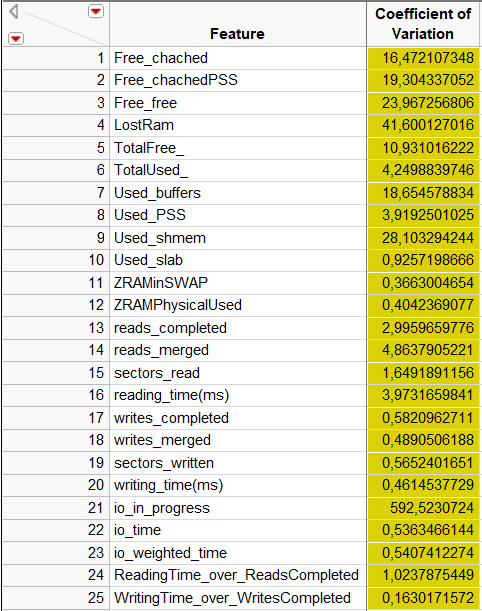
\includegraphics[width=.7\linewidth,keepaspectratio]{cov.png}
  \caption{Cofficenti di Variazione(CV)}
  \label{}
\end{figure}

\subsection{PCA}
In questa fase è stata applicata la
\textbf{\textit{PCA(Principal Component Analysis)}}
la quale trasforma un workload con parametri correlati in uno contente parametri
non correlati.\\
L'utilizzo della PCA in questa è necessario anche per la fase successiva, in
quanto il clustering funziona meglio se i parametri non sono correlati.\\
Per effettuare la PCA si è fatto utilizzo del tool \textit{\textbf{JMP}}, nella
figura è riportato l'output.\\

\begin{figure}[!htbp]
	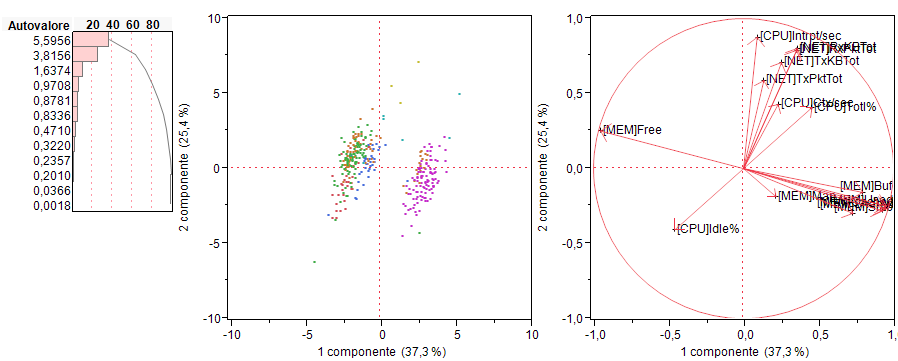
\includegraphics[width=\linewidth,keepaspectratio]{pca.png}
  \caption{Risultato PCA}
  \label{}
\end{figure}

\begin{figure}[!htbp]
	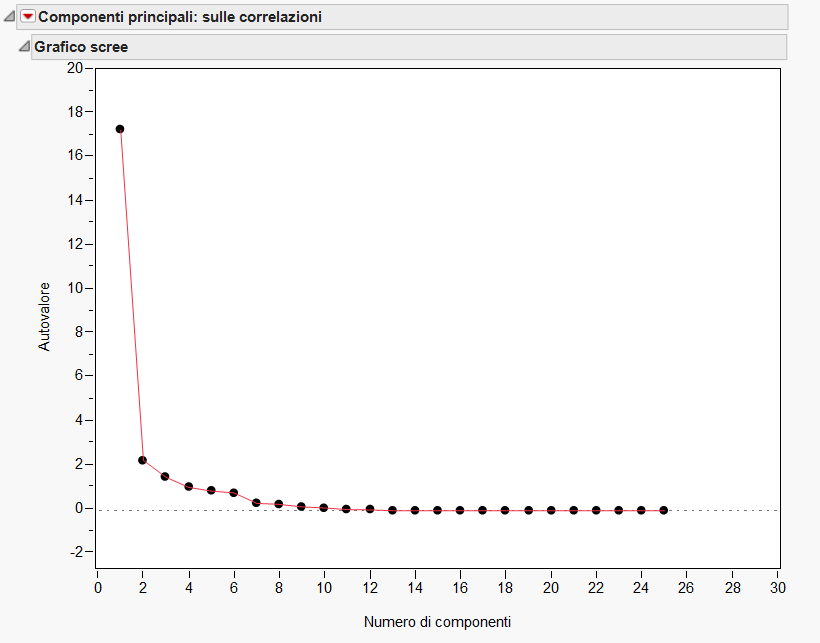
\includegraphics[width=\linewidth,keepaspectratio]{grafico_scree.png}
  \caption{Grafico Scree}
  \label{grafico_scree}
\end{figure}

Considerando il grafico in \figurename~\ref{grafico_scree}, rappresentate
sull'asse delle x il numero di componenti principali e sull'asse delle y
gli autovalori, per scegliere il numero di componenti principali ci si
posiziona nel ginocchio della curva, poichè in quel punto ci si assicura che
aggiungendo un'ulteriore componente la varianza conservata non aumenta
significativamente.\\
Quindi si è scelto di considerare 6 componenti principali.\\

\begin{figure}[!htbp]
	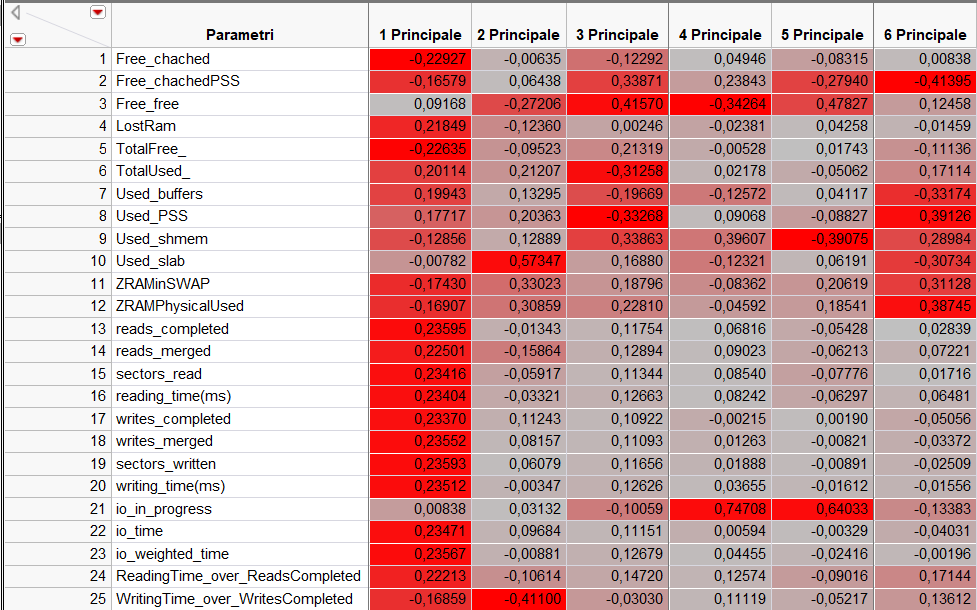
\includegraphics[width=\linewidth,keepaspectratio]{autovettori.png}
  \caption{Autovettori}
  \label{}
\end{figure}

Nella figura sono evidenziati in rosso i parametri che hanno contribuito maggiormente,
in segno positivo o negativo, alla creazione delle componenti principali scelti.\\
In particolare:
\begin{itemize}
  \item \textbf{\textit{Principale 1:}} \textit{Free\_chached, LostRam, TotalFree,
  reads\_completed, reads\_merged, sectors\_read, reading\_time(ms),
  writes\_completed, writes\_merged, sector\_written, writing\_time(ms),
  io\_time, io\_weighted\_time e ReadingTime\_over\_ReadsCompleted};
  \item \textbf{\textit{Principale 2:}} \textit{Used\_slab e WritingTime\_over\_WritesCompleted};
  \item \textbf{\textit{Principale 3:}} \textit{Free\_free, TotalUsed e Used\_PSS};
  \item \textbf{\textit{Principale 4:}} \textit{io\_in\_progress};
  \item \textbf{\textit{Principale 5:}} \textit{Used\_shmem};
  \item \textbf{\textit{Principale 6:}} \textit{Free\_chachedPSS, Used\_buffers e Used\_PSS, ZRamPhysicalUsed};
\end{itemize}

\subsection{Clustering}
In questa fase è stato effettuate un operazione di clustering sul risultato
ottenuto nello step precedente.\\
La tecnica di clasterizzazione scelta è di tipo gerarchico agglomerativo,
in particolare è stata utilizzata la metrica di word
per l'aggregazione dei cluster.\\
In figura è riportato il dendogramma risultante.\\


\begin{figure}[!htbp]
	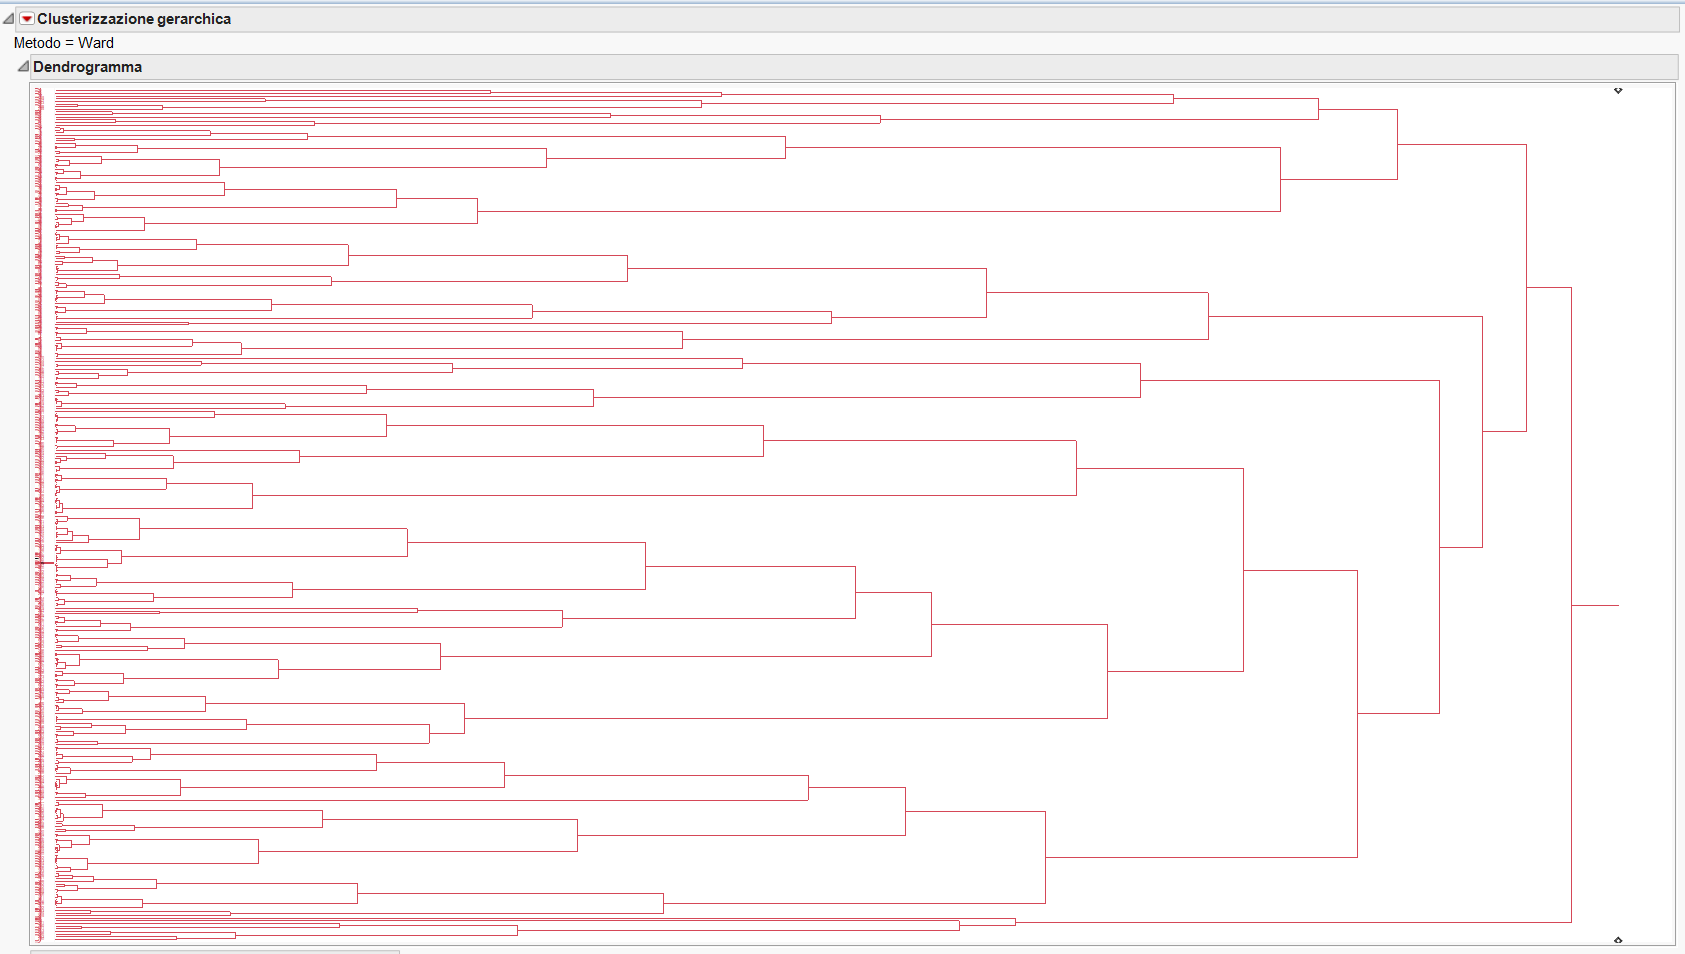
\includegraphics[width=\linewidth,keepaspectratio]{dendogramma.png}
  \caption{Dendogramma}
  \label{dendogramma}
\end{figure}

Facendo riferimento alla \figurename~\ref{dendogramma}, si può scegliere il numero
di cluster posizionandosi nel ginocchio della curva rappresentante le distanze tra cluster.\\
\clearpage
In maniera analoga si può scegliere il numero di cluster utilizzando il criterio
clusterizzazione cubica, riportato il \figurename~\ref{ccc}, scegliendo il numero
cluster utilizzando la regola del massimo salto.\\

\begin{figure}[htbp]
\centering
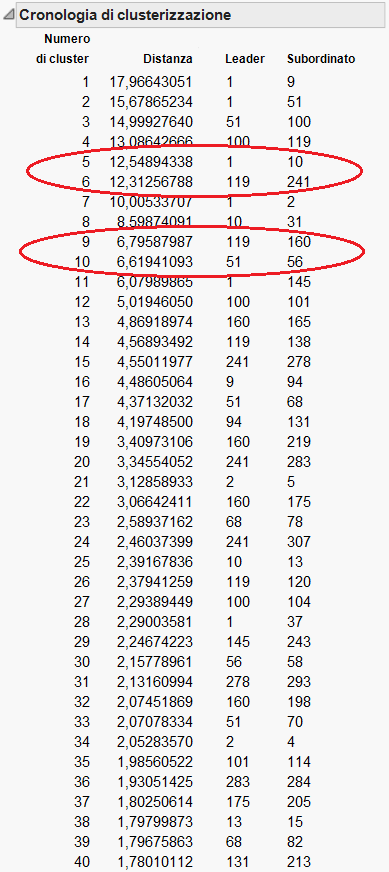
\includegraphics[width=50mm]{gerarchia_clustering.png}% "%" necessario
\qquad\qquad
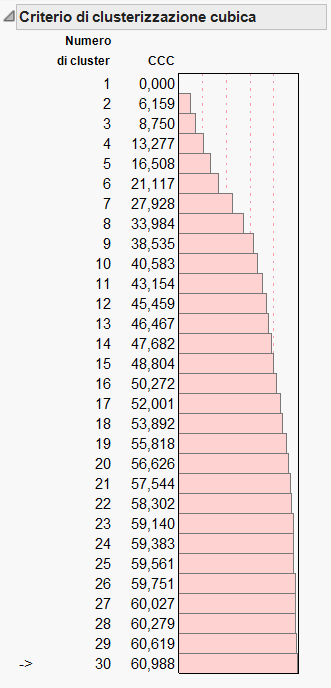
\includegraphics[width=50mm]{ccc.png}
\caption{Gerarchia clustering e Criterio di Clasterizzazione Cubica}
\label{ccc}
\end{figure}

Sulla base dei criteri sopra descritti si è scelto di considerare 6 cluster, per
la generazione del workload sitnetico si è scelto di estrarre randomicamente
un esperimento da ogni cluster.\\
\clearpage
\section{Conclusioni}
Dagli step descritti abbiamo ottenuto un Workload sintetico,
ma non si è detto quanta varianza si è conservato.\\
Per calcolare quanta varianza abbiamo conservato bisogna calcolare quanta
ne abbiamo conservato in ogni ogni step.\\
Per la PCA la varianza conservata è 95,702\%, valore ottenuto da JMP.\\
Per il clustering non si può  utlizzare la varianza ma bisogna utilizzare la devianza
poichè essa è indipendente dal grado di libertà dei cluster i quali hanno diverse
dimensioni.\\
Per il calcolo della percentuale di devianza conservata utilizzando il clustering
si è calcolata la devianza del workload sottoposto a PCA, in quanto il clustering è stato
effettuato successivamente.\\
La devianza conservata è calcolata come la somma della  devianza inter-cluster
e intra-cluster, poichè utilizzando il clustering si perde varianza inter-cluster
e scegliendo un campione per ogni cluster si perde varianza infra-cluster.\\
Nella seguente figure è riportata la devianza del workload sottoposto a PCA.\\

\begin{figure}[!htbp]
	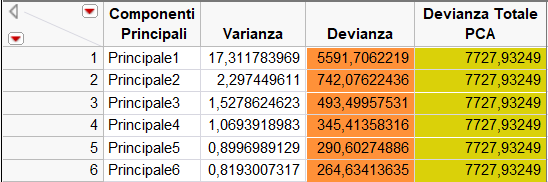
\includegraphics[width=.7\linewidth,keepaspectratio]{devianza_pca.png}
  \caption{Devianza PCA}
  \label{}
\end{figure}
\clearpage

Nella seguente figura è riportato la devianza inter-cluster.\\

\begin{figure}[!htbp]
	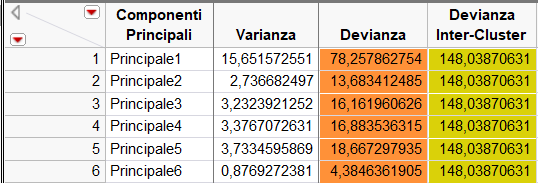
\includegraphics[width=.7\linewidth,keepaspectratio]{devianza_inter_clustering.png}
  \caption{Devianza Inter-Cluster}
  \label{}
\end{figure}

Nella seguente figura è riportato la devianza intra-cluster.\\

\begin{figure}[!htbp]
	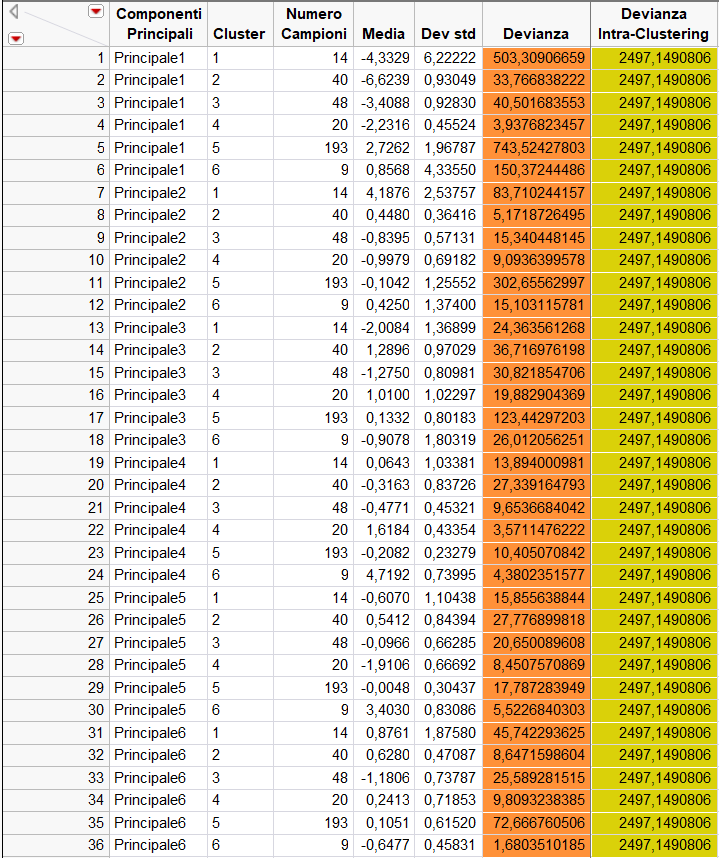
\includegraphics[width=.7\linewidth,keepaspectratio]{devianza_intra_clustering.png}
  \caption{Devianza Intra-Cluster}
  \label{}
\end{figure}
\clearpage

Quindi per il calcolo della percentuale di devianza conservata utilizzando la
tecnica di clasterizzazione si utilizzata la seguente formula:
$$1-{devianza_{inter\_cluster}+devianza_{intra\_cluster}\over {devianza_{pca}}}$$

In tabella è riportato la percentuale di devianza persa/conservata utilizzando
il clustering.\\

\vspace{5 mm}

\begin{tabular}{|c|c|}
\hline
\textbf{Devianza PCA}	& 7727,93249 \\
\hline
\textbf{Devianza Clustering(intra-cluster+inter-cluster)}	& 2645,1867 \\
\hline
\textbf{Percentuale devianza persa clusterizzando}	& 34,22\% \\
\hline
\textbf{Percentuale devianza conservata clusterizzando}	& 65,78\% \\
\hline
\textbf{Significatività PCA} &	95,70\% \\
\hline
\end{tabular}

\vspace{5 mm}

Nella seguente figure è riportata la percentuale di varianza persa/conservata del
workload sintetico.\\

\vspace{5 mm}

\begin{tabular}{c|c|c|}
 & \textbf{Conservata} & \textbf{Perse} \\
 \hline
 \textbf{Workload Reale} & 100,00\% &	0,00\% \\
 \hline
 \textbf{PCA} &	95,70\%	& 4,30\% \\
 \hline
 \textbf{Clustering} &	62,95\%	& 37,05\% \\
 \hline
\end{tabular}

\vspace{5 mm}

In conclusione utilizzando 6 componenti principali e 6 cluster si perde il 37,05\%
di significatività rispetto al workload reale.
